\chapter{Python scripts}

\section{\acs{wkt} visualisation}
\label{sec:wktVisualisation}
\begin{minted}{python}
import matplotlib.pyplot as plt
import rdflib

levels = [
    "inst:level_1xS3BCk291UvhgP2dvNMKI",
    "inst:level_1xS3BCk291UvhgP2dvNMQJ",
    "inst:level_1xS3BCk291UvhgP2dvNsgp",
    "inst:level_1xS3BCk291UvhgP2dvNtSE"
]

data = {}

for level in levels:
    g = rdflib.Graph()
    qres = g.query("""
      PREFIX props: <https://w3id.org/props#>
      PREFIX rdf: <http://www.w3.org/1999/02/22-rdf-syntax-ns#>
      PREFIX bot: <https://w3id.org/bot#>
      PREFIX inst: <https://172.16.10.122:8080/projects/1001/>
      SELECT ?s ?o
      WHERE {
        SERVICE <http://localhost:7200/repositories/duplex-v1> {
          ?s props:hasSimple2DBoundary ?o .
          ?s rdf:type bot:Space .
          """ + str(level) + """ bot:hasSpace ?s.
        }
      }
      LIMIT 100
      """)
    rooms = {}
    for row in qres:
        polygon_string = row.o.n3()
        polygon_string = polygon_string.replace('POLYGON (', '').replace('()', '').replace(')', '').replace(
            '"', '').replace('^^<http://www.opengis.net/ont/geosparql#wktLiteral>', '')
        coordinate_pairs = polygon_string.split(', ')
        coordinates = [(int(pair.split(' ')[0]), int(pair.split(' ')[1]))
                       for pair in coordinate_pairs]
        row.o.n3()
        room = row.s.n3().replace(
            '<https://172.16.10.122:8080/projects/1001/', '').replace('>', '')
        rooms[room] = coordinates
    data[level] = rooms


def showLevel(level):
    level = data[level]
    plt.figure()
    for room, polygon in level.items():
        xs, ys = zip(*polygon)
        plt.plot(xs, ys, label=room)
    plt.axis('equal')
    plt.legend(bbox_to_anchor=(1, 1))
    plt.show()
\end{minted}

\begin{minted}{python}
for level in levels:
    print(level)
    print(data[level].keys())
    showLevel(level)
\end{minted}

\begin{minted}[bgcolor=white]{output}
texttt{inst:level_1xS3BCk291UvhgP2dvNMKI
dict_keys(['room_1xS3BCk291UvhgP2dvNvkw', 'room_1xS3BCk291UvhgP2dvNvk7', 'room_1xS3BCk291UvhgP2dvNvk0', 'room_1xS3BCk291UvhgP2dvNvkD', 'room_1xS3BCk291UvhgP2dvNcNR', 'room_1xS3BCk291UvhgP2dvNcOa', 'room_1xS3BCk291UvhgP2dvNcOX', 'room_1xS3BCk291UvhgP2dvNcOY', 'room_1xS3BCk291UvhgP2dvNb9h', 'room_1xS3BCk291UvhgP2dvNbEa'])}
\end{minted}

\begin{figure}[H]
  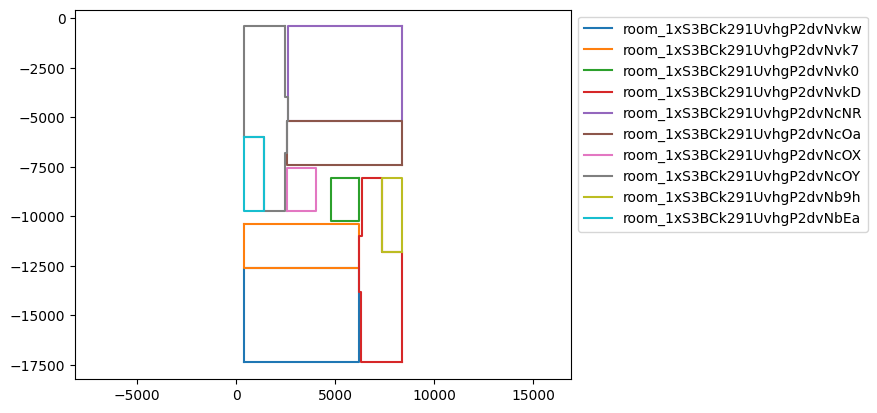
\includegraphics[width=\textwidth]{figures/png/WKT output/output1.png}
\end{figure}

\begin{minted}[bgcolor=white]{output}
inst:level_1xS3BCk291UvhgP2dvNMQJ
dict_keys(['room_1xS3BCk291UvhgP2dvNvkK', 'room_1xS3BCk291UvhgP2dvNvkG', 'room_1xS3BCk291UvhgP2dvNvkT', 'room_1xS3BCk291UvhgP2dvNvkU', 'room_1xS3BCk291UvhgP2dvNcOe', 'room_1xS3BCk291UvhgP2dvNcOq', 'room_1xS3BCk291UvhgP2dvNcOn', 'room_1xS3BCk291UvhgP2dvNcOo', 'room_1xS3BCk291UvhgP2dvNdjF', 'room_1xS3BCk291UvhgP2dvNdjS'])
\end{minted}

\begin{figure}[H]
  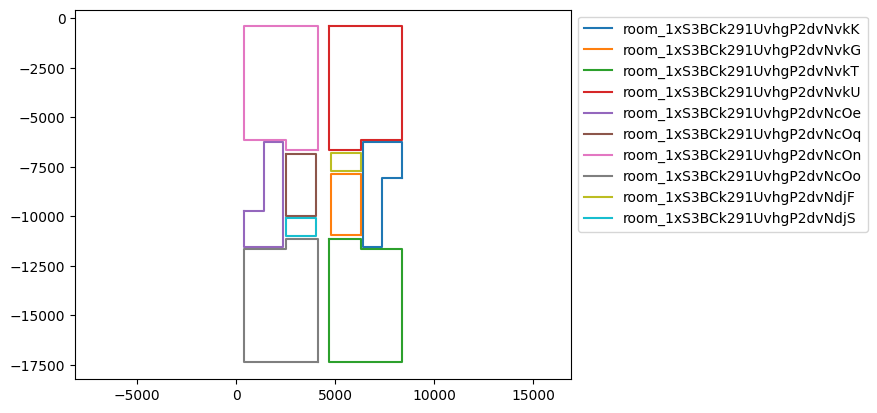
\includegraphics[width=\textwidth]{figures/png/WKT output/output2.png}
\end{figure}

\begin{minted}[bgcolor=white]{output}
inst:level_1xS3BCk291UvhgP2dvNtSE
dict_keys(['room_1xS3BCk291UvhgP2dvNbq0'])
\end{minted}

\begin{figure}[H]
  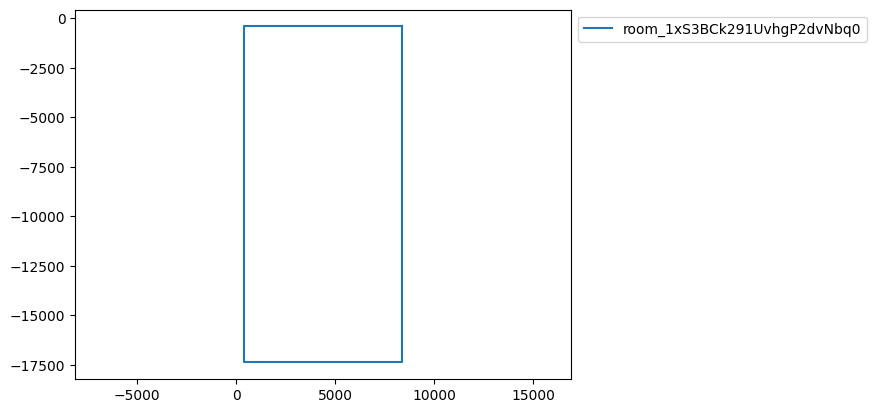
\includegraphics[width=\textwidth]{figures/png/WKT output/output3.png}
\end{figure}

\begin{minted}{python}
def showRoom(level, room):
    polygon = data[level][room]
    plt.figure()
    xs, ys = zip(*polygon)
    plt.plot(xs, ys)
    plt.axis('equal')
    plt.show()
showRoom("inst:level_1xS3BCk291UvhgP2dvNMKI", "room_1xS3BCk291UvhgP2dvNvkw")
\end{minted}

\begin{figure}[H]
  \centering
  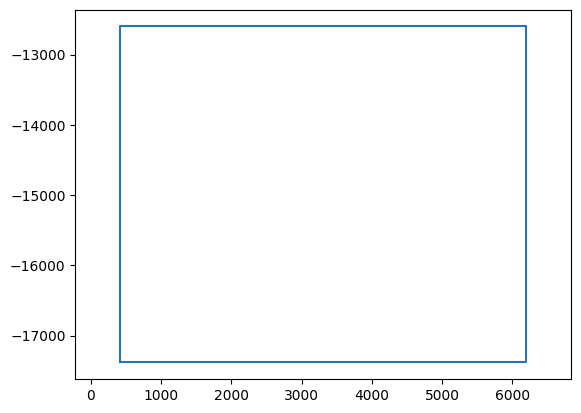
\includegraphics[width=0.7\textwidth]{figures/png/WKT output/output4.png}
\end{figure}

\section{Geometry extraction}
\label{sec:pyhtonExtraction}
\begin{minted}{python}
  import rdflib
  
  g = rdflib.Graph()
  qres = g.query("""
  PREFIX props: <https://w3id.org/props#>
  PREFIX rdf: <http://www.w3.org/1999/02/22-rdf-syntax-ns#>
  PREFIX bot: <https://w3id.org/bot#>
  PREFIX fog: <https://w3id.org/fog#>
  PREFIX xsd: <http://www.w3.org/2001/XMLSchema#>
  SELECT ?s ?o
  WHERE {
    SERVICE <http://localhost:7200/repositories/duplex-v1> {
      ?s fog:asObj ?o .
      filter(datatype(?o)=xsd:string)
    }
  }
  # LIMIT 10
  """)
  
  for row in qres:
      name = row.s.replace("https://172.16.10.122:8080/projects/1001/", "")
      name = name.replace("%", "-") # for github user content
      extention = ".obj"
      directory = "out/"
      fileName = directory + name + extention
      file = open(fileName, "w")
      file.write(row.o)
      file.close()
  \end{minted}